
\section{Auswertung}
\subsection{Bestimmung der Brennweiten durch Messung der Gegenstands- und Bildweite}
Die gemessenen Werte für die Bild- und Gegenstandsweiten der beiden Sammellinsen sind
in Tabelle \ref{tab:Sb} und Tabelle \ref{tab:Su} dargestellt. Die Brennweiten lassen sich nach
\ref{} berechnen.
\begin{table}
\centering
\caption{Sammellinse f=150mm}
\label{tab:Sb}
\begin{tabular}{S S S}
\toprule
{$g$ in $\si{\centi\meter}$} & {$b$ in $\si{\centi\meter}$} & {$f$ in $\si{\centi\meter}$}\\
\midrule
17 & 101,5 & 14,561 \\
19 & 60,8 & 14,476 \\
21 & 48,8 & 14,646 \\
23 & 41,2 & 14,760 \\
25 & 34,8 & 14,548 \\
27 & 31,2 & 14,474 \\
29 & 28,9 & 14,475\\
31 & 27,0 & 14,431 \\
33 & 26,0 & 14,542 \\
35 & 24,5 & 14,412\\
\bottomrule
\end{tabular}
\end{table}

\begin{table}
\centering
\caption{Sammellinse f=50mm}
\label{tab:Su}
\begin{tabular}{S S S}
\toprule
{$g$ in $\si{\centi\meter}$} & {$b$ in $\si{\centi\meter}$} & {$f$ in $\si{\centi\meter}$}\\
\midrule
44 & 6,0 & 5,280 \\
42 & 6,1 & 5,326 \\
40 & 6,1 & 5,293 \\
38 & 6,2 & 5,330 \\
36 & 6,3 & 5,362 \\
34 & 6,4 & 5,386 \\
32 & 6,4 & 5,333 \\
30 & 6,5 & 5,342 \\
28 & 6,5 & 5,275 \\
26 & 6,7 & 5,327\\
\bottomrule
\end{tabular}
\end{table}
\begin{figure}
  \centering
  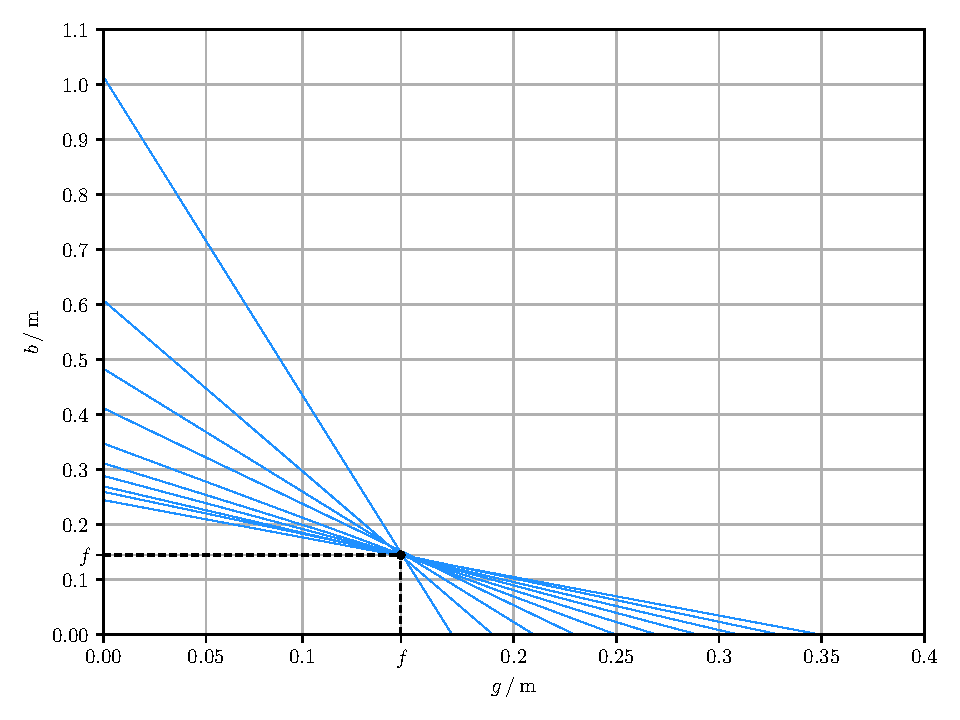
\includegraphics[scale=0.7]{Plot.pdf}
  \caption{Darstellung für die Brennweite f=150mm}
  \label{fig:bb}
\end{figure}
\begin{figure}
  \centering
  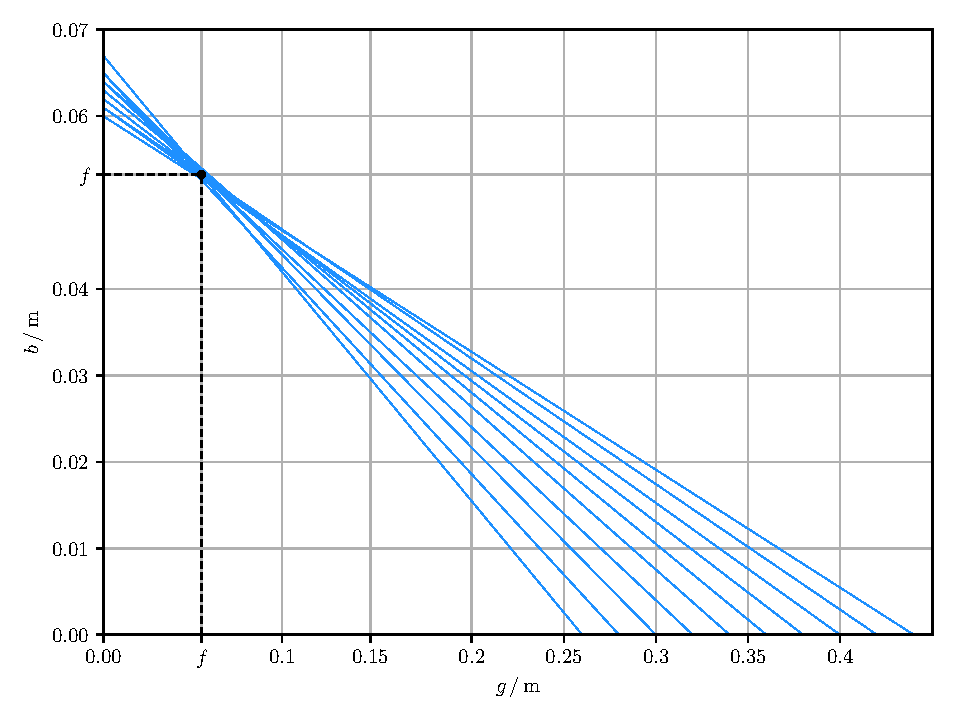
\includegraphics[scale=0.7]{Plot2.pdf}
  \caption{Darstellung für die Brennweite f=50mm'}
  \label{fig:plotbu}
\end{figure}
Für die beiden Brennweiten ergeben sich die folgenden theoretische Werte
\begin{align}
  f\ua{150mm} &= \SI{145(3)}{\milli\meter}\\
  f\ua{50mm} &= \SI{53(1)}{\milli\meter}.
\end{align}
Insgesamt folgt aus den theoretischen und experimentellen Werten die Brennweiten von
\begin{align}
  \overline{f}\ua{150mm} &= \SI{145,165(165)}{\milli\meter}
\end{align}
und
\begin{align}
  \overline{f}\ua{50mm} &= \SI{53,125(125)}{\milli\meter}.
\end{align}

\subsection{Bestimmung der Brennweite nach der Methode von Bessel}
Die Messwerte der Bildweiten $b_{1}$ und $b_{2}$,der Gegenstandsweiten $g_{1}$ und $g_{2}$ und
dem Abstand $e$ zwischen Schirm und Gegenstand sind aus Tabelle \ref{tab:bessel} zu entnehmen.
Wie bei der ersten Messung, wurde auch für diesen Teil des Versuchs eine Sammellinse mit der Brennweite
$f=150$\,mm verwendet. Mithilfe von Formel () lässt sich der Linsenabstand ermitteln.
Die Fehler für f werden nicht weiter berücksichtigt, da diese um zwei Größenordnungen kleiner sind.
\begin{table}
\centering
\caption{Messdaten der Methode nach Bessel}
\label{tab:bessel}
\begin{tabular}{S S S S S S S}
\toprule
{$e$ in $\si{\centi\meter}$} & {$b_1$ in $\si{\centi\meter}$} & {$b_2$ in $\si{\centi\meter}$} & {$g_1$ in $\si{\centi\meter}$} & {$g_2$ in $\si{\centi\meter}$}&
{$d$ in $\si{\centi\meter}$} & {$f$ in $\si{\centi\meter}$} \\
\midrule
71 & 51,4 & 20,5 & 19,6 & 50,5 & 30,90\pm0,90 & 14,388\\
73 & 53,3 & 19,9 & 19,7 & 53,1 & 33,40\pm0,20 & 14,430\\
75 & 56,0 & 19,6 & 19,0 & 55,4 & 36,40\pm0,60 & 14,333\\
77 & 58,2 & 19,5 & 18,8 & 57,5 & 38,70\pm0,70 & 14,387\\
79 & 60,3 & 19,2 & 18,7 & 59,8 & 41,10\pm0,50 & 14,404\\
81 & 62,4 & 18,8 & 18,6 & 62,3 & 43,65\pm0,15 & 14,369\\
83 & 64,8 & 18,8 & 18,2 & 64,2 & 46,00\pm0,60 & 14,377\\
85 & 66,6 & 18,6 & 18,4 & 66,4 & 48,00\pm0,20 & 14,474\\
87 & 69,0 & 18,5 & 18,0 & 68,5 & 50,50\pm0,50 & 14,422\\
89 & 71,0 & 18,3 & 18,0 & 70,7 & 52,70\pm0,30 & 14,449\\
\bottomrule
\end{tabular}
\end{table}
\newline
Die Brennweite wird anschließend zu
\begin{align}
  f = \SI{144,03(20)}{\centi\meter}
\end{align}
gemittelt. Der Mittelwert und die Standardabweichung errechnen sich dabei durch
\begin{equation}
  \bar{x} = \frac{1}{n} \sum{x_n}
  \label{eqn:Mittelwert}
\end{equation}
und
\begin{equation}
\upsigma = \frac{1}{\sqrt{n}} \sqrt{\frac{\sum{(x_n - \bar{x})^2}}{n-1} }.
\label{eqn:Standardabweichung}
\end{equation}
\newline
Die Werte für die chromatischen Abberration sind in Tabelle \ref{tab:besselblau} für blaues
Licht und in Tabelle \ref{tab:besselrot} für rotes Licht aufgetragen. Die Berechnung des Linsenabstands
und der Brennweite werden wie oben berechnet.
\begin{table}
\centering
\caption{blau}
\label{tab:besselblau}
\begin{tabular}{S S S S S S S}
\toprule
{$e$ in $\si{\centi\meter}$} & {$b_1$ in $\si{\centi\meter}$} & {$b_2$ in $\si{\centi\meter}$} & {$g_1$ in $\si{\centi\meter}$} & {$g_2$ in $\si{\centi\meter}$} & {$d$ in $\si{\centi\meter}$} & {$f$ in $\si{\centi\meter}$}\\
\midrule
75 & 56,0 & 19,9 & 19,0 & 55,1 & 24,0\pm1,1 & 18,630\\
73 & 53,6 & 19,8 & 19,4 & 53,2 & 34,6\pm0,8 & 18,131\\
71 & 50,9 & 20,6 & 20,1 & 50,4 & 30,3\pm0,5 & 17,643\\
69 & 48,8 & 20,8 & 20,2 & 48,2 & 28,0\pm0,6 & 17,149\\
67 & 46,2 & 21,5 & 20,8 & 45,4 & 24,7\pm0,7 & 16,658 \\
\bottomrule
\end{tabular}
\end{table}

\begin{table}
\centering
\caption{blau}
\label{tab:besselrot}
\begin{tabular}{S S S S S S S}
\toprule
{$e$ in $\si{\centi\meter}$} & {$b_1$ in $\si{\centi\meter}$} & {$b_2$ in $\si{\centi\meter}$} & {$g_1$ in $\si{\centi\meter}$} & {$g_2$ in $\si{\centi\meter}$}\
& {$d$ in $\si{\centi\meter}$} & {$f$ in $\si{\centi\meter}$}\\
\midrule
67 & 45,7 & 21,7 & 21,3 & 45,3 & 24,0\pm0,6 & 16,660\\
69 & 48,7 & 20,8 & 20,3 & 48,2 & 28,9\pm0,5 & 17,145\\
71 & 51,1 & 20,4 & 19,9 & 50,6 & 30,7\pm0,5 & 17,642\\
73 & 53,5 & 19,9 & 19,5 & 53,1 & 33,6\pm0,4 & 18,135\\
75 & 55,6 & 20,0 & 19,4 & 55,0 & 35,6\pm0,6 & 18,631 \\
\bottomrule
\end{tabular}
\end{table}
Daraus folgt für die Brennweiten
\begin{align}
  f\ua{blau} &= \SI{176,42(348)}{\milli\meter}\\
  f\ua{rot} &= \SI{175,89(489)}{\milli\meter}.
\end{align}

\subsection{Bestimmung des Brennweite des Linsensystems nach der Methode von Abbe}
Die Messwerte für das Linsenpaar sind in Tabelle \ref{tab:abbe} zu finden. Zusätzlich
wurde mit Gleichung () die unterschiedlichen V berechnet.
\newline
Die Gegenstandsgröße G beträgt 3\,cm.
\begin{table}
\centering
\caption{Messdaten der Methode nach Abbe}
\label{tab:abbe}
\begin{tabular}{S S S S}
\toprule
{Bildgröße $B$ in $\si{\centi\meter}$} & {$b'$ in $\si{\centi\meter}$} & {$g'$ in $\si{\centi\meter}$} & {V}\\
\midrule
2,0 & 14,95 & 9,05 & 0,67 \\
1,3 & 14,05 & 12,05 & 0,43 \\
1,0 & 13,95 & 14,15 & 0,33 \\
0,9 & 13,85 & 16,25 & 0,30 \\
0,8 & 13,45 & 18,65 & 0,27 \\
0,7 & 13,45 & 18,65 & 0,23 \\
0,6 & 13,45 & 20,65 & 0,20 \\
0,6 & 12,05 & 24,75 & 0,20 \\
0,5 & 13,25 & 26,85 & 0,20 \\
0,5 & 12,95 & 30,05 & 0,20\\
\bottomrule
\end{tabular}
\end{table}
\newline
Anhand der linearen Regressionen in Abbildungen \ref{fig:plotg} und \ref{fig:plotb} werden die
gesuchten Größen h und f bestimmt. Diese werden mit Formel () und () bestimmt.
\begin{figure}
  \centering
  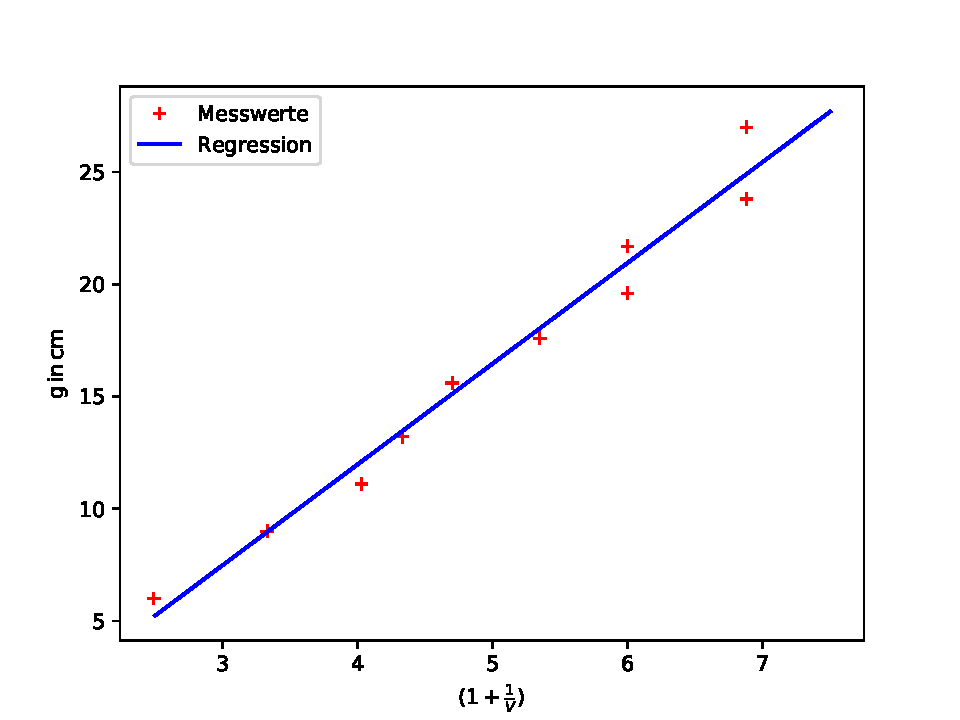
\includegraphics[scale=0.7]{plotg.pdf}
  \caption{Lineare Regression für g'}
  \label{fig:plotg}
\end{figure}
\begin{figure}
  \centering
  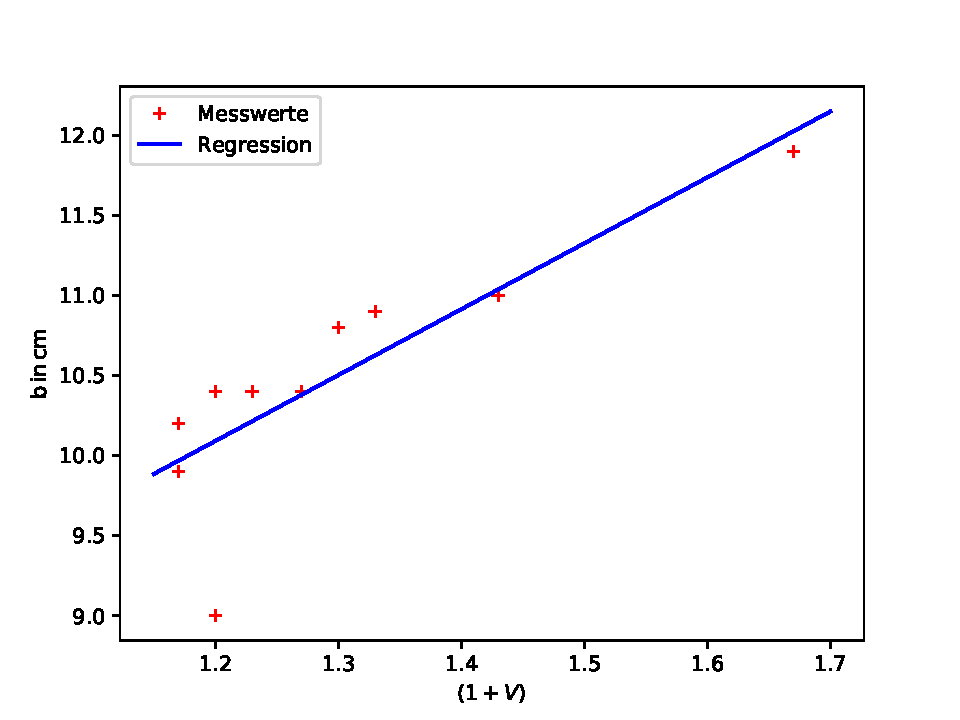
\includegraphics[scale=0.7]{plotb.pdf}
  \caption{Lineare Regression für b'}
  \label{fig:plotb}
\end{figure}
\newpage
Für die Lage der Hauptebenen im Abstand zum Referenzpunkt A ergeben sich die Werte
\begin{align*}
  h &= -\SI{60(13)}{\milli\meter}\\
  h' &= \SI{52(12)}{\milli\meter}.
\end{align*}
Für die Brennweiten folgt
\begin{align*}
  f\ua{g}&= \SI{44,9(25)}{\milli\meter}\\
  f\ua{b} &= \SI{41(10)}{\milli\meter}.
\end{align*}
Aus den beiden Brennweiten ergibt sich ein Mittelwert von
\begin{align*}
  f\ua{Mittel} &= \SI{42,95(195)}{\milli\meter}.
\end{align*}
\newpage
\section{Diskussion}
Die Brennweiten bestimmt über die Gegenstands- und Bildweiten sind relativ genau gemessen worden.
Bei der Sammellinse mit einer Brennweite von f=150\,mm beträgt die prozentuale Abweichung 3,3 \%
im Vergleich zu der bestimmten Brennweite f=145\,mm. Die geringe prozentuale Abweichung ist auch gut
in der Grafik erkennbar. Hier stimmt der Brennpunkt relativ genau mit dem Schnittpunkt der eingezeichneten Geraden
überein.\newline
Bei der zweiten Sammellinse mit f=50\,mm wurde eine Brennweite von f=53\,mm besimmt, was einer Abweichung von 5,6 \% entspricht.
Die etwas größere Abweichung von dem Herstellerwert und dem berechneten Brennpunkt ist im Graphen zu erkennen.
Die Geraden haben keinen gemeinsamen Schnittpunkt.
\newline
Die chromatische Abberation hingegen konnte nicht dem erwarteten Ergebnis gerecht werden. Der Brennpunkt des blauen Lichts
ist weiter von dem weißen Licht entfernt als der rote. Eigentlich hätte der Brennpunkt des blauen Lichts aufgrund
der stärken Brechung näher an der Linse sein müssen. Dieses unerwartete Ergebnis könnte auf den geringen Kontrast
des blauen Lichts zurückgeführt werden. Hier war es besonders schwierig einen scharfen Punkt zu finden.
\newline
Bei der Messung der Brennweiten eines Linsensystems nach Abbe wurden die Bildgrößen auf dem Schirm jeweils mit einem
Geodreieck gemessen. Deshalb konnten die Bildgrößen zwar ungefähr bestimmt werden, allerdings sind diese händisch nicht exakt
messbar.
\newline
Der Abstand der beiden Hauptachsen zum Brennpunkt ist etwas erhöht. Mit dem Geodreieck wurde ein Abstand von 3,05\,cm bestimmt.
Allerdings lässt sich feststellen, dass der Referenzpunkt relativ mittig gewählt wurde. Die berechneten Brennweiten sind
recht genau.
\newline
Insgesamt lässt sich sagen, dass während des gesamten Versuchs die Definiton des scharfen Bildes eine Ermässensache war.
Außerdem war es schwierig einzelne Entfernung abzulesen, da die Skala zur dunklen Wand gerichtet war. Diese beiden,
doch relativ großen Fehlerquellen, lassen die Abweichung der bestimmten Brennweiten erklären.

